\documentclass[11pt]{article}
\usepackage[round,sort&compress]{natbib}
\setcitestyle{aysep={}}
\usepackage{newpxtext,newpxmath}
\usepackage[T1]{fontenc}
\usepackage{hyperref}
\usepackage{graphicx}
\usepackage{amsmath}
\usepackage[left]{lineno}
\linenumbers

\topmargin 0.0cm
\oddsidemargin 0.2cm
\textwidth 16cm 
\textheight 21cm
\footskip 1.0cm

\newcommand{\perexpcorrmaps}{S1}
\newcommand{\perexptaskrecon}{S2}
\newcommand{\perexptaskreconseparated}{S3}
\newcommand{\freqpower}{S4}
\newcommand{\networkpower}{S5}
\newcommand{\suppstats}{S6}

% Include your paper's title here

\title{A Gaussian process model of human electrocorticographic data} 
\author{
  Lucy L. W. Owen$^{1}$,
  Tudor A. Muntianu$^{1}$,
  Andrew C. Heusser$^{1, 2}$, \\
  Patrick Daly$^{3}$,
  Katherine Scangos$^{3}$, and
  Jeremy R. Manning$^{1\ast}$\\\\
$^{1}$Department of Psychological and Brain Sciences, Dartmouth College,\\
Hanover, NH 03755, USA\\
$^{2}$Akili Interactive,\\
Boston, MA 02110, USA\\
$^{3}$Weill Institute for Neurosciences, University of California, San Francisco,\\
San Francisco, CA 94121, USA}

\date{}

\begin{document} 

\baselineskip24pt
\maketitle 

\begin{abstract}
  We present a model-based method for inferring full-brain neural
  activity at millimeter-scale spatial resolutions and
  millisecond-scale temporal resolutions using standard human
  intracranial recordings.  Our approach assumes that different
  people's brains exhibit similar correlational structure, and that
  activity and correlation patterns vary smoothly over space.  One can
  then ask, for an arbitrary individual's brain: given recordings from
  a limited set of locations in that individual's brain, along with
  the observed spatial correlations learned from other people's
  recordings, how much can be inferred about ongoing activity at
  \textit{other} locations throughout that
  individual's brain?  We show that our approach generalizes across
  people and tasks, thereby providing a person- and task-general means
  of inferring high spatiotemporal resolution full-brain neural
  dynamics from standard low-density intracranial recordings.
  \\\\
  \footnotesize{\textbf{Keywords: Electrocorticography (ECoG),
      intracranial electroencephalography (iEEG), local field
      potential (LFP), epilepsy, maximum likelihood estimation,
      Gaussian process regression}}
\end{abstract}

\section*{Introduction}
Modern human brain recording techniques are fraught with
compromise~\citep{SejnEtal14}.  Commonly used approaches include
functional magnetic resonance imaging (fMRI), scalp
electroencephalography (EEG), and magnetoencephalography (MEG).  For
each of these techniques, neuroscientists and electrophysiologists
must choose to optimize spatial resolution at the cost of temporal
resolution (e.g., as in fMRI) or temporal resolution at the cost of
spatial resolution (e.g., as in EEG and MEG).  A less widely used
approach (due to requiring work with neurosurgical patients) is to
record from electrodes implanted directly onto the cortical surface
(electrocorticography; ECoG) or into deep brain structures
(intracranial EEG; iEEG).  However, these intracranial approaches also
require compromise: the high spatiotemporal resolution of
intracranial recordings comes at the cost of substantially reduced
brain coverage, since safety considerations limit the number of
electrodes one may implant in a given patient's brain.  Further, the
locations of implanted electrodes are determined by clinical, rather
than research, needs.

An increasingly popular approach is to improve the effective spatial
resolution of MEG or scalp EEG data by using a geometric approach
called \textit{beamforming} to solve the biomagnetic or bioelectrical
inverse problem~\citep{Sarv87}.  This approach entails using detailed
brain conductance models (often informed by high spatial resolution
anatomical MRI images) along with the known sensor placements
(localized precisely in 3D space) to reconstruct brain signals
originating from theoretical point sources deep in the brain (and far
from the sensors).  Traditional beamforming approaches must overcome
two obstacles.  First, the inverse problem beamforming seeks to solve
has infinitely many solutions.  Researchers have made traction towards
constraining the solution space by assuming that signal-generating
sources are localized on a regularly spaced grid spanning the brain
and that individual sources are small relative to their distances to
the sensors~\citep{Snyd91, BailEtal01, HillEtal05}.  The second, and in
some ways much more serious, obstacle is that the magnetic fields
produced by external (noise) sources are substantially stronger than
those produced by the neuronal changes being sought (i.e., at deep
structures, as measured by sensors at the scalp).  This means that
obtaining adequate signal quality often requires averaging the
measured responses over tens to hundreds of responses or trials~\citep[e.g., see review by][]{HillEtal05}.

Another approach to obtaining high spatiotemporal resolution
neural data has been to collect fMRI and EEG data simultaneously.
Simultaneous fMRI-EEG has the potential to balance the high spatial
resolution of fMRI with the high temporal resolution of scalp EEG,
thereby, in theory, providing the best of both worlds.  In practice,
however, the signal quality of both recordings suffers substantially
when the two techniques are applied simultaneously~\citep[e.g., see review by][]{HustEtal12}.  In addition, the experimental designs that are
ideally suited to each technique individually are somewhat at odds.
For example, fMRI experiments often lock stimulus presentation
events to the regularly spaced image acquisition time (TR), which
maximizes the number of post-stimulus samples.  By contrast, EEG
experiments typically employ jittered stimulus presentation times to
maximize the experimentalist's ability to distinguish electrical brain
activity from external noise sources such as from 60 Hz alternating
current power sources.

The current ``gold standard'' for precisely localizing signals and
sampling at high temporal resolution is to take (ECoG or iEEG)
recordings from implanted electrodes (but from a limited set of
locations in any given brain).  This begs the following question: what
can we infer about the activity exhibited by the rest of a person's
brain, given what we learn from the limited intracranial recordings we
have from their brain and additional recordings taken from
\textit{other} people's brains?  Here we develop an approach, which we
call \textit{SuperEEG}\footnote{The term ``SuperEEG''
  was coined by Robert J. Sawyer in his popular science fiction novel
  \textit{The Terminal Experiment}~\cite{Sawy95}.  SuperEEG is a
  fictional technology that measures ongoing neural activity
  throughout the entire living human brain with perfect precision and
  at arbitrarily high spatiotemporal resolution.}, based on Gaussian
process regression~\citep{Rasm06}.  SuperEEG entails using data from
multiple people to estimate activity patterns at arbitrary locations
in each person's brain (i.e., independent of their electrode
placements).  We test our SuperEEG approach using two large datasets
of intracranial recordings~\citep{SedeEtal03, SedeEtal07a, SedeEtal07b,
  MannEtal11, MannEtal12, EzzyEtal17, HoraEtal17, KragEtal17,
  KuceEtal17, LinEtal17, SoloEtal18, WeidEtal18, EzzyEtal18,
  KuceEtal18}.  We show that the SuperEEG algorithm recovers signals
well from electrodes that were held out of the training dataset.  We
also examine the factors that influence how accurately activity may be
estimated (recovered), which may have implications for electrode
design and placement in neurosurgical applications.

\section*{Approach}
The SuperEEG approach to inferring high temporal resolution full-brain
activity patterns is outlined and summarized in
Figure~\ref{fig:methods}. We describe (in this section) and evaluate
(in \textit{Results}) our approach using a two large previously
collected datasets comprising multi-session intracranial recordings.
Dataset 1 comprises multi-session recordings taken from 6876
electrodes implanted in the brains of 88 epilepsy
patients~\citep{SedeEtal03, SedeEtal07a, SedeEtal07b, MannEtal11,
  MannEtal12}.  Each recording session lasted from 0.2--3~h (total
recording time: 0.3--14.2~h; Fig.~\suppstats E).  During each
recording session, the patients participated in a free recall list
learning task, which lasted for up to approximately 1~h.  In addition,
the recordings included ``buffer'' time (the length varied by patient)
before and after each experimental session, during which the patients
went about their regular hospital activities (confined to their
hospital room, and primarily in bed).  These additional activities
included interactions with medical staff and family, watching
television, reading, and other similar activities.  For the purposes
of the Dataset 1 analyses presented here, we aggregated all data
across each recording session, including recordings taken during the
main experimental task as well as during non-experimental time.  We
used Dataset 1 to develop our main SuperEEG approach, and to examine
the extent to which SuperEEG might be able to generate task-general
predictions.  Dataset 2 comprised multi-session recordings from 4436
electrodes implanted in the brains of 40 epilepsy
patients~\citep{EzzyEtal17, HoraEtal17, KragEtal17, KuceEtal17,
  LinEtal17, SoloEtal18, WeidEtal18, EzzyEtal18, KuceEtal18}.  Each
recording session lasted from 0.4--2.2~h (total recording time:
0.4--6.6~h; Fig.~\suppstats K).  Whereas Dataset 1 included recordings
taken as the patients participated in a variety of activities, Dataset
2 included recordings taken as each patient performed each of two
specific experimental memory tasks: a random word list free recall
task (Experiment 1) and a categorized word list free recall task
(Experiment 2).  We used Dataset 2
to further examine the ability of SuperEEG to generalize its
predictions within versus across tasks.  Figure~\suppstats~provides
additional information about both datasets.

\begin{figure}
  \centering
  \includegraphics[width=\textwidth]{figs/methods}
  \caption{\textbf{Methods overview.}  \textbf{A.~Electrode
      locations.}  Each dot reflects the location of a single
    electrode implanted in the brain of a Dataset 1 patient.  A
    held-out recording location from one patient is indicated in red,
    and the patient's remaining electrodes are indicated in black.
    The electrodes from the remaining patients are colored by
    $k$-means cluster (computed using the full-brain correlation model
    shown in Panel D).  \textbf{B.~Radial basis function kernel.}
    Each electrode contributed by the patient (black) weights on the
    full set of locations under consideration (all dots in Panel A,
    defined as $\bar{R}$ in the text).  The weights fall off with
    positional distance (in MNI space) according to an RBF.
    \textbf{C.~Per-patient correlation matrices.}  After computing the
    pairwise correlations between the recordings from each patient's
    electrodes, we use RBF-weighted averages to estimate correlations
    between all locations in $\bar{R}$.  We obtain an estimated
    full-brain correlation matrix using each patient's
    data. \textbf{D.~Merged correlation model.}  We combine the
    per-patient correlation matrices (Panel C) to obtain a single
    full-brain correlation model that captures information contributed
    by every patient.  Here we have sorted the rows and columns to
    reflect $k$-means clustering labels~\citep[using
    $k$=7;][]{YeoEtal11}, whereby we grouped locations based on their
    correlations with the rest of the brain (i.e., rows of the matrix
    displayed in the panel).  The boundaries denote the cluster
    groups.  The rows and columns of Panel C have been sorted using
    the Panel D-derived cluster labels.  \textbf{E.~Reconstructing activity
      throughout the brain.}  Given the observed recordings from the
    given patient (shown in black; held-out recording is shown in
    blue), along with a full-brain correlation model (Panel D), we
    use Equation~\ref{eqn:reconstruction} to reconstruct the most
    probable activity at the held-out location (red).}
  \label{fig:methods}
\end{figure}

We first applied fourth order Butterworth notch filter to remove 60 Hz
($\pm$ .5 Hz) line noise from every recording (from every electrode).
Next, we downsampled the recordings (regardless of the original
sample rate) to 250 Hz.  (This downsampling step served to both
normalize for differences in sampling rates across patients and to
ease the computational burden of our subsequent analyses.)  We then
excluded any electrodes that showed putative epileptiform activity.
Specifically, we excluded from further analysis any electrode that
exhibited an maximum kurtosis of 10 or greater across all of that
patient's recording sessions.  We also excluded any patients with
fewer than 2 electrodes that passed this criteria, as the SuperEEG
algorithm requires measuring correlations between 2 or more electrodes
from each patient.  For Dataset 1, this yielded clean recordings from
4168 electrodes implanted throughout the brains of 67 patients
(Fig.~\ref{fig:methods}A); for Dataset 2, this yielded clean
recordings from 5023 electrodes from 78 patients.  Each individual
patient contributes electrodes from a limited set of brain locations,
which we localized in a common space~\citep[MNI152;][]{GrabEtal06}; an
example Dataset 1 patient's 54 electrodes that passed the above
kurtosis threshold test are highlighted in black and red.

The recording from a given electrode is maximally informative about
the activity of the neural tissue immediately surrounding its
recording surface.  However, brain regions that are distant from the
recording surface of the electrode also contribute to the recording,
albeit (ceteris paribus) to a much lesser extent.  One mechanism
underlying these contributions is volume conduction.  The precise rate
of falloff due to volume conduction (i.e., how much a small volume of
brain tissue at location $x$ contributes to the recording from an
electrode at location $\eta$) depends on the size of the recording
surface, the electrode's impedance, and the conductance profile of the
volume of brain between $x$ and $\eta$.  As an approximation of this
intuition, we place a Gaussian radial basis function (RBF) at the
location $\eta$ of each electrode's recording surface
(Fig.~\ref{fig:methods}B).  We use the values of the RBF at any brain
location $x$ as a rough estimate of how much structures around $x$
contributed to the recording from location $\eta$:
\begin{align}
  \mathrm{rbf}(x|\eta,\lambda) & =
  \mathrm{exp}\left\{ -\frac{||x - \eta||^2}{\lambda} \right\},\label{eqn:rbf}
\end{align}
where the width variable $\lambda$ is a parameter of the algorithm
(which may in principle be set according to location-specific tissue
conductance profiles) that governs the level of spatial smoothing.  In
choosing $\lambda$ for the analyses presented here, we sought to
maximize spatial resolution (which implies a small value of $\lambda$)
while also maximizing the algorithm's ability to generalize to any
location throughout the brain, including those without dense electrode
coverage (which implies a large value of $\lambda$).  Here we set
$\lambda = 20$, guided in part by our prior work~\citep{MannEtal14b,
  MannEtal18}, and in part by examining the brain coverage with
non-zero weights achieved by placing RBFs at each electrode location
in Dataset 1 and taking the sum (across all electrodes) at each voxel
in a 4~mm$^3$ MNI brain.  (We then held $\lambda$ fixed for our
analyses of Dataset 2.)  We note that this value could in theory be
further optimized, e.g., using cross validation or a formal
model~\citep[e.g.,][]{MannEtal18}.

A second mechanism whereby a given region $x$ can contribute to the
recording at $\eta$ is through (direct or indirect) anatomical
connections between structures near $x$ and $\eta$.  Although
anatomical and functional correlations can differ
markedly~\citep[e.g.,][]{AdacEtal12, HoneEtal09, GoniEtal14}, we use temporal
correlations in the data to estimate these anatomical
connections~\citep{BeckEtal18}.  Let $\bar{R}$ be the set of locations
at which we wish to estimate local field potentials, and let
$R_{s} \subseteq \bar{R}$ be set of locations at which we observe local
field potentials from patient $s$ (excluding the electrodes that did
not pass the kurtosis test described above). In the analyses below we
define $\bar{R} = \cup_{s=1}^S R_s$.  We can calculate the expected
inter-electrode correlation matrix for patient $s$, where
$C_{s,k}(i,j)$ is the correlation between the time series of voltages
for electrodes $i$ and $j$ from subject $s$ during session $k$, using:

\begin{align}
  \bar{C}_{s} &=
  \mathrm{r}(\frac{1}{n}(\sum_{k=1}^{n}\mathrm{z}(C_{s,k}))),\label{eqn:inter_corr}~\mathrm{where}\\
\mathrm{z}(r) &= \frac{\log(1+r) - \log(1 - r)}{2}~\mathrm{is~the~Fisher}~z \mathrm{-transformation~and}\label{eqn:fishersz}\\
\mathrm{z}^{-1}(z) = \mathrm{r}(z) &= \frac{\exp(2z) - 1}{\exp(2z) + 1}\mathrm{~is~its~inverse}.\label{eqn:invfishersz}
\end{align}
Next, we use Equation~\ref{eqn:rbf} to construct a number of
to-be-estimated locations by number of patient electrode locations
weight matrix, $W_s$.  Specifically, $W_s$ approximates how informative the
recordings at each location in $R_s$ are in reconstructing activity at
each location in $\bar{R}$, where the contributions fall off with an RBF according to
the distances between the corresponding locations:

\begin{align}
W_s(i, j) = \mathrm{rbf}(i|j,\lambda)\label{eqn:weight_matrix}.
\end{align}

Given this weight matrix, $W_s$,
and the observed inter-electrode correlation matrix for patient $s$,
$\bar{C}_{s}$, we can estimate the correlation matrix for all locations in
$\bar{R}$ ($\hat{C}_s$; Fig.~\ref{fig:methods}C) using:

\begin{align}
\hat{N}_{s}(x,y) & = { \sum_{i = 1}^{| R_{s}|}\sum_{j=1}^{i-1} W(x,i) \cdot W(y,j)\cdot \mathrm{z}(\bar{C}_{s}(i,j))}\label{eqn:subj_corrmat_num}\\
 \hat{D}_{s}(x,y) & = \sum_{i = 1}^{| R_{s}|}\sum_{j=1}^{i-1} W(x,i)
                    \cdot W(y,j). \label{eqn:subj_corrmat_den}\\
 \hat{C}_s &= \mathrm{r}\left( \frac{\hat{N}_{s}}{\hat{D}_{s}} \right)
             \label{eqn:subj_corrmat}.
\end{align}
After estimating the numerator ($\hat{N}_{s}$) and denominator
($\hat{D}_{s}$) placeholders for each $\hat{C}_{s}$, we aggregate these
estimates across the $S$ patients to obtain a single expected full-brain
correlation matrix ($\hat{K}$; Fig.~\ref{fig:methods}D):
\begin{align}
 \hat{K} = \mathrm{r} \left(  \frac{\sum_{s=1}^S  \hat{N}_{s}}{\sum_{s=1}^S \hat{D}_{s}}\right).\label{eqn:corrmat}
\end{align}
Intuitively, the numerators capture the general structures of the
patient-specific estimates of full-brain correlations, and the
denominators account for which locations were near the implanted
electrodes in each patient.  To obtain $\hat{K}$, we compute a
weighted average across the estimated patient-specific full-brain
correlation matrices, where patients with observed electrodes near a
particular set of locations in $\hat{K}$ contribute more to the
estimate.

Having used the multi-patient data to estimate a full-brain
correlation matrix at the set of locations in $\bar{R}$ that we wish
to know about, we next use $\hat{K}$ to estimate activity patterns
everywhere in $\bar{R}$, given observations at only a subset of
locations in $\bar{R}$ (Fig.~\ref{fig:methods}E).

Let $\alpha_s$ be the set of indices of patient $s$'s electrode locations in
$\bar{R}$ (i.e., the locations in $R_s$), and let $\beta_s$ be the set of indices of all other
locations in $\bar{R}$. In other words, $\beta_s$ reflects the locations
in $\bar{R}$ where we did not observe a recording for patient $s$
(these are the recording locations we will want to fill in using SuperEEG).
We can sub-divide $\hat{K}$ as follows:

\begin{align}
\hat{K}_{\beta_s,\alpha_s} &= \hat{K}(\beta_s,\alpha_s),~\mathrm{and}\label{eqn:Kba}\\
\hat{K}_{\alpha_s,\alpha_s} &= \hat{K}(\alpha_s,\alpha_s)\label{eqn:Kaa}.
\end{align}
Here $\hat{K}_{\beta_s, \alpha_s}$ represents the correlations between
the ``unknown'' activity at the locations indexed by $\beta_s$ and the
observed activity at the locations indexed by $\alpha_s$, and
$\hat{K}_{\alpha_s, \alpha_s}$ represents the correlations between the
observed recordings (at the locations indexed by $\alpha_s$).

Let $Y_{s,k,\alpha_s}$ be the number-of-timepoints ($T$) by
$\left|\alpha_s\right|$ matrix of (observed) voltages from the electrodes in
$\alpha_s$ during session $k$ from patient $s$. Then we can estimate the
voltage from patient $s$'s $k^{th}$ session at the locations in
$\beta_s$ using~\cite{Rasm06}:

\begin{align}
\hat{Y}_{s,k,\beta_s} &= ((\hat{K}_{\beta_s,\alpha_s}\cdot\hat{K}_{\alpha_s,\alpha_s}^{-1})\cdot Y_{s,k,\alpha_s}^\mathrm{T})^\mathrm{T}.\label{eqn:reconstruction}
\end{align}
This equation is the foundation of the SuperEEG algorithm.  Whereas we
observe recordings only at the locations indexed by $\alpha_s$,
Equation~\ref{eqn:reconstruction} allows us to estimate the recordings
at all locations indexed by $\beta_s$, which we can define \textit{a priori}
to include any locations we wish, throughout the brain.  This yields
estimates of the time-varying voltages at \textit{every} location in
$\bar{R}$, provided that we define $\bar{R}$ in advance to include the
union of all of the locations in $R_s$ and all of the locations
at which we wish to estimate recordings (i.e., a timeseries of
voltages).

We designed our approach to be agnostic to electrode impedances, as
electrodes that do not exist do not have impedances.  Therefore our
algorithm recovers voltages in standard deviation ($z$-scored) units
rather than attempting to recover absolute voltages. (This property
reflects the fact that $\hat{K}_{\beta_s, \alpha_s}$ and
$\hat{K}_{\alpha_s, \alpha_s}$ are correlation matrices rather than
covariance matrices.)  Also, we note that
Equation~\ref{eqn:reconstruction} requires computing a $T$ by $T$
matrix, which can become computationally intractable when $T$ is very
large (e.g., an example patient in Dataset 1, $T =
12786750$). However, because Equation~\ref{eqn:reconstruction} is time
invariant, we may compute $Y_{s,k,\beta_s}$ in a piecewise
manner by filling in $Y_{s,k,\beta_s}$ one row at a time (using the
corresponding samples from $Y_{s, k, \alpha_s}$).

The SuperEEG algorithm described above and in Figure~\ref{fig:methods}
allows us to estimate, up to a constant scaling factor, local field
potentials (LFPs) for each patient at all arbitrarily chosen locations
in the set $\bar{R}$, \textit{even if we did not record that patient's
  brain at all of those locations}.  We next turn to an evaluation of
the accuracy of those estimates.

\section*{Results}
We used a cross-validation approach to test the accuracy with which
the SuperEEG algorithm reconstructs activity throughout the brain.
For each patient in turn, we estimated full-brain correlation matrices
(Eqn.~\ref{eqn:corrmat}) using data from all of the \textit{other}
patients. This step ensured that the data we were reconstructing could
not also be used to estimate the between-location correlations that
drove the reconstructions via Equation~\ref{eqn:reconstruction}
(otherwise the analysis would be circular).  For that held-out
patient, we held out each electrode in turn.  We used
Equation~\ref{eqn:reconstruction} to reconstruct activity at the
held-out electrode location, using the correlation matrix learned from
all other patients' data as $\hat{K}$, and using activity recorded
from the other electrodes from the held-out patient as
$Y_{s, k, \alpha_s}$.  We then asked: how closely did each of the
SuperEEG-estimated recordings at those electrodes match the observed
recordings from those electrodes (i.e., how closely did the estimated
$\hat{Y}_{s, k, \beta_s}$ match the observed $Y_{s, k, \beta_s}$)?

We used this general approach to
quantify the algorithm's performance across the full dataset. For each held-out electrode, from each held-out patient in turn, we
computed the average correlation (across recording sessions) between
the SuperEEG-reconstructed voltage traces and the observed voltage
traces from that electrode.  For this analysis we set $\bar{R}$ to be
the union of all electrode locations across all patients.  This
yielded a single correlation coefficient for each electrode location
in $\bar{R}$, reflecting how well the SuperEEG algorithm was able to
recover the recording at that location by incorporating data across
patients (black histogram in Fig.~\ref{fig:corrmap}A, map in
Fig.~\ref{fig:corrmap}C).  The observed distribution of correlations
was centered well above zero (mean: 0.51; $t$-test comparing mean of
distribution of $z$-transformed average patient correlation coefficients
to 0: $t(66) = 23.55, p < 10^{-10}$), indicating that the SuperEEG algorithm
recovers held-out activity patterns substantially better than random
guessing.

As a stricter benchmark, we compared the quality of these
across-participant reconstructions (i.e., computed using a correlation
model learned from other patients' data) to reconstructions generated
using a correlation model trained using the in-patient's data.  In
other words, for this within-patient benchmark analysis we estimated
$\hat{C}_{s}$ (Eqn.~\ref{eqn:subj_corrmat}) for each patient in turn,
using recordings from all of that patient's electrodes except at the
location we were reconstructing.  These within-patient reconstructions
serve as an estimate of how well data from all of the other electrodes
from that single patient may be used to estimate held-out data from
the same patient.  This allows us to ask how much information about
the activity at a given electrode might be inferred through (a) volume
conductance or other sources of ``leakage'' from activity patterns
measured from the patient's other electrodes and (b) across-electrode
correlations learned from that single patient.  As shown in
Figure~\ref{fig:corrmap}A (gray histogram), the distribution of
within-patient correlations was centered well above zero (mean: 0.32;
$t$-test comparing mean of distribution of $z$-transformed average
patient correlation coefficients to 0: $t(66) = 15.16, p < 10^{-10}$).
However, the across-patient correlations were substantially higher
($t$-test comparing average $z$-transformed within versus across
patient electrode correlations: $t(66) = 9.17, p < 10^{-10}$).  This
is an especially conservative test, given that the across-patient
SuperEEG reconstructions exclude (from the correlation matrix
estimates) all data from the patient whose data is being
reconstructed.  We repeated each of these analyses on a second
independent dataset and found similar results
(Fig.~\ref{fig:corrmap}B, D; within versus across reconstruction
accuracy: $t(77) = 11.25, p < 10^{-10}$). We also replicated this result
separately for each of the two experiments from Dataset 2
(Fig.~\perexpcorrmaps).  This overall finding, that reconstructions of
held-out data using correlation models learned from \textit{other}
patient's data yield higher reconstruction accuracy than correlation
models learned from the patient whose data is being reconstructed, has
two important implications.  First, it implies that distant electrodes
provide additional predictive power to the data reconstructions beyond
the information contained solely in nearby electrodes.  (This follows
from the fact that each patient's grid, strip, and depth electrodes
are implanted in a unique set of locations, so for any given electrode
the closest electrodes in the full dataset tend to come from the
same patient.)  Second, it implies that the spatial correlations
learned using the SuperEEG algorithm are, to some extent, similar
across people.

%correlations by brain area, distribution of correlations
\begin{figure}
  \centering
  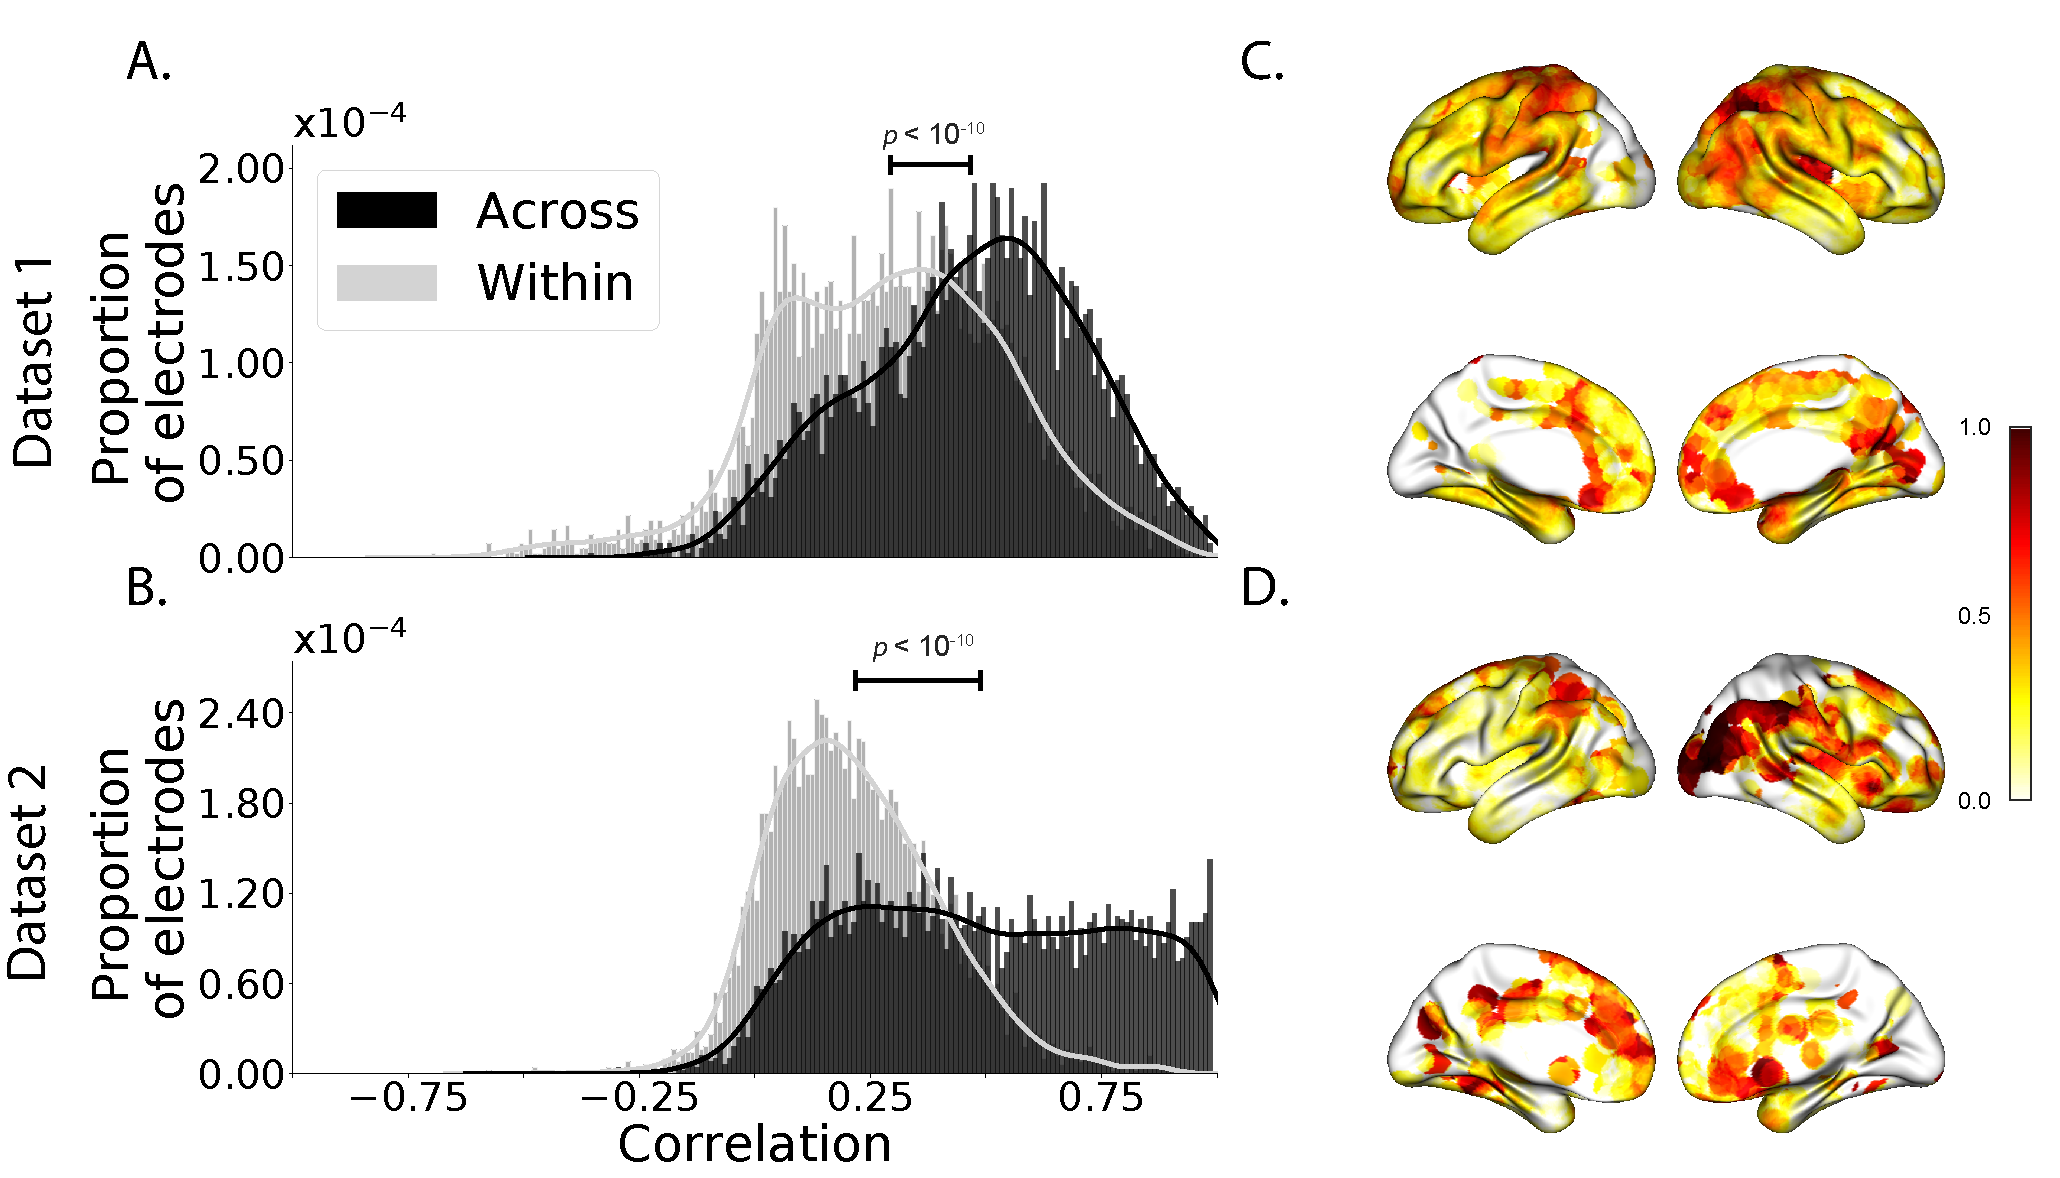
\includegraphics[width=\textwidth]{figs/corrmap}
  \caption{\textbf{Reconstruction quality across all electrodes in two
      ECoG datasets.}  \textbf{A. Distributions of correlations
      between observed versus reconstructed activity by electrode, for
      Dataset 1.}  The across-patient distribution (black) reflects
    reconstruction accuracy (correlation) using a correlation model
    learned from all but one patient's data, and then applied to that
    held-out patient's data.  The within-patient distribution (gray)
    reflects performance using a correlation model learned from the same
    patient who contributed the to-be-reconstructed electrode.
    \textbf{B. Distributions of correlations for Dataset 2.}  This
    panel is in the same format as Panel A, but reflects results
    obtained from Dataset 2.  The histograms aggregate data across
    both Dataset 2 experiments; for results broken down by experiment
    see Figure~\perexptaskreconseparated. \textbf{C.--D.  Reconstruction
      performance by location.} The colors denote the average across-session
    correlation, using the across-patient correlation model, between
    the observed and reconstructed activity at the given electrode
    location projected to the cortical surface~\citep{CombEtal19}.}
  \label{fig:corrmap}
\end{figure}

The recordings we analyzed from Dataset 1 comprised data collected as
the patients performed a variety of (largely idiosyncratic) tasks
throughout each day's recording session.  That we observed reliable
reconstruction accuracy across patients suggests that the spatial
correlations derived from the SuperEEG algorithm are, to some extent,
similar across tasks.  We tested this finding more directly using
Dataset 2.  In Dataset 2, the recordings were limited to times when
each patient was participating in one of two experiments.  Experiment
1 is a random-word list free recall task; Experiment 2 is a
categorized list free recall task (24 patients particpated in both).  We wondered whether a correlation
model learned from data from one experiment might yield good
predictions of data from the other experiment.  Further, we wondered
about the extent to which it might be beneficial or harmful to combine
data across tasks.

To test the task-specificity of the SuperEEG-derived correlation
models, we restricted the dataset to the 24 patients that participated
in both experiments and repeated the above within- and across-patient cross validation
procedures separately for Experiment 1 and Experiment 2 data from
Dataset 2.  We then compared the reconstruction accuracies for held-out
electrodes, for models trained within versus across the two
experiments, or combining across both experiments
(Fig.~\perexptaskrecon).  In every case we found that across-patient
models trained using data from all other patients out-performed
within-patient models trained on data only from the subject
contributing the given electrode ($t$s$(23) > 6.50, p$s$ < 10^{-5}$).  All
reconstruction accuracies also reliably exceeded chance performance
($t$s$(23) > 8.00, p$s$ < 10^{-8}$).  Average reconstruction accuracy was
highest for the across-patient models limited to data from the same
experiment (mean accuracy: $0.68$); next-highest for the
models that combined data across both experiments (mean
accuracy: $0.61$); and lowest for models trained across tasks (mean
accuracy: $0.47$).  This result also held for each of the Dataset 2
experiments individually (Fig.~\perexptaskreconseparated).  Taken
together, these results indicate that there are reliable commonalities
in the spatial correlations of full-brain activity across tasks, but
that there are also reliable differences in these spatial correlations
across tasks.  Whereas reconstruction accuracy benefits from
incorporating data from other patients, reconstruction accuracy is
highest when constrained to within-task data, or data that includes a
variety of tasks (e.g., Dataset 1, or combining across the two Dataset
2 experiments).

Although both datasets we examined provide good full-brain coverage
(when considering data from every patient; e.g.\
Fig.~\ref{fig:corrmap}C, D), electrodes are not placed uniformly
throughout the brain.  For example, electrodes are more likely to be
implanted in regions like the medial temporal lobe (MTL), and are
rarely implanted in occipital cortex (Fig.~\ref{fig:density}A, B).
Separately for each dataset, for each voxel in the 4~mm$^3$ voxel
MNI152 brain, we computed the proportion of electrodes in the dataset
that were contained within a 20 MNI unit radius sphere centered on
that voxel.  We defined the \textit{density} at that location as this
proportion.  Across Datasets 1 and 2, the electrode placement
densities were similar (correlation by voxel:
$r = 0.6, p < 10^{-10}$).  We wondered whether regions with good
covererage might be associated with better reconstruction accuracy
(e.g. Fig.~\ref{fig:corrmap}C and D indicate that many electrodes in the
MTL have relatively high reconstruction accuracy, and occipital
electrodes tend to have relatively low reconstruction accuracy).  To
test whether this held more generally across the entire brain, for
each dataset we computed the electrode placement density for each
electrode from each patient (using the proportion of \textit{other}
patients' electrodes within 20 MNI units of the given electrode).  We
then correlated these density values with the across-patient
reconstruction accuracies for each electrode.  We found a negative
correlation between reconstruction accuracy and density for Dataset 1,
but was unreliable for Dataset 2 (Dataset 1: $r = -0.21, p = 0.05$; Dataset 2:
$r = -0.30, p = 0.15$).  This indicates that the reconstruction
accuracies we observed are not driven by sampling density, but
rather may also reflect higher order properties of neural dynamics
such as functional correlations between distant
voxels~\citep{BetzEtal17b}.

\begin{figure}
  \centering
  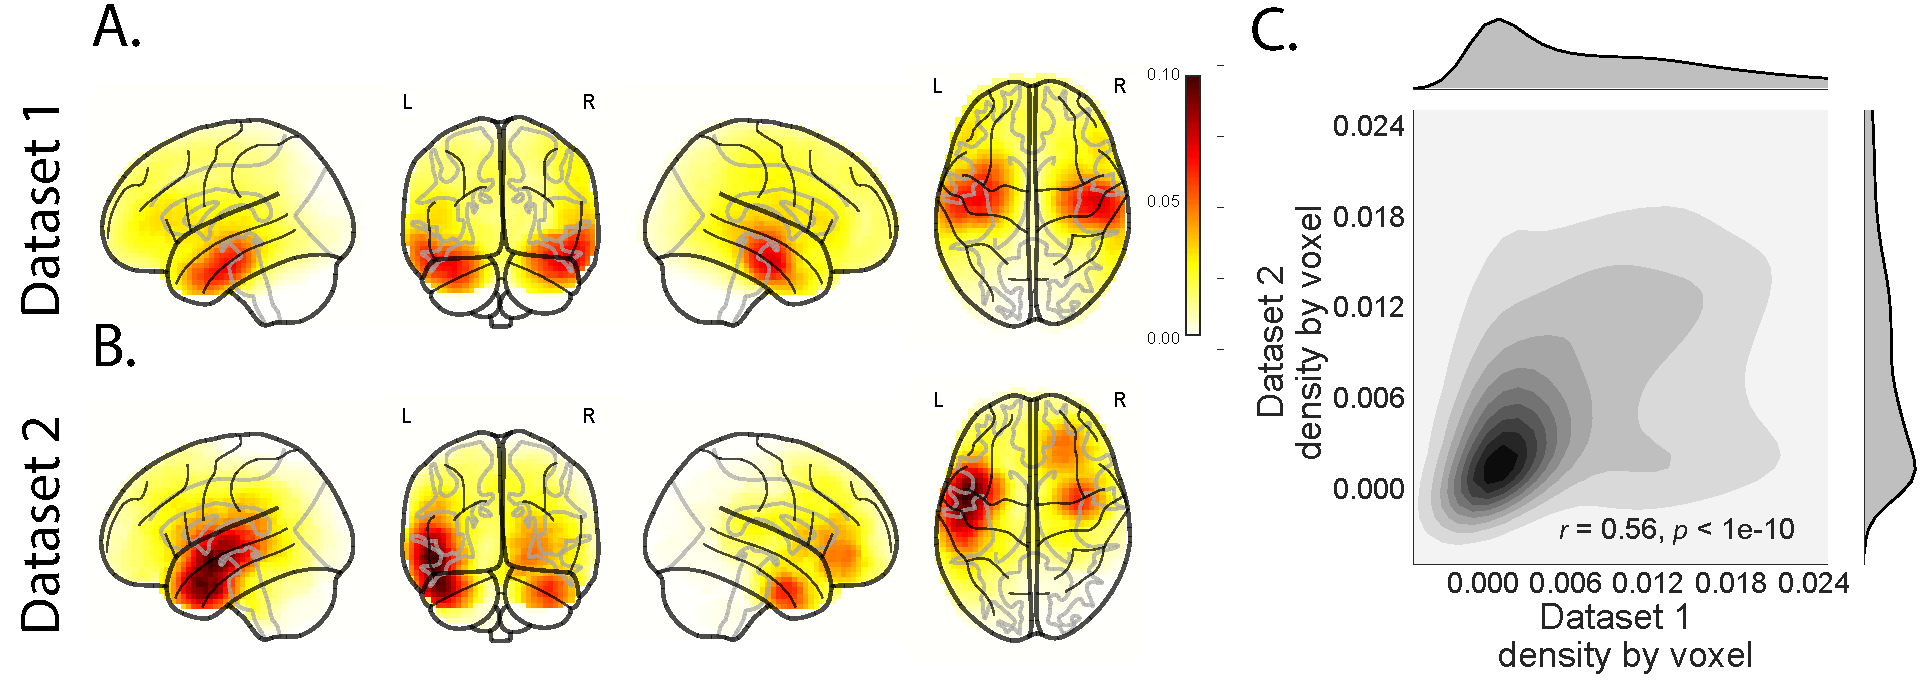
\includegraphics[width=\textwidth]{figs/density}
  \caption{\textbf{Electrode sampling density by location.}
    \textbf{A.~Electrode sampling density by voxel in Dataset 1.} Each
    voxel is colored by the proportion of total electrodes in the
    dataset that are
    located within a 20~MNI unit radius sphere centered on the given
    voxel.  \textbf{B.~Electrode sampling density by voxel in Dataset
      2.}  This panel displays the sampling density map for Dataset 2,
    in the same format as Panel A.  \textbf{C.~Correspondence in
      sampling density by voxel across Datasets 1 and 2.}  The
    two-dimensional histogram displays the by-voxel densities in the
    two Datasets, and the one-dimensional histograms display the
    proportions of voxels in each dataset with the given density
    value.  The correlation reported in the panel is across voxels in
    the 4~mm$^3$ MNI brain.}
  \label{fig:density}
\end{figure}

In neurosurgical applications where one wishes to infer full-brain
activity patterns, can our framework yield insights into where the
electrodes should be placed?  A basic assumption of our approach (and
of most prior ECoG work) is that electrode recordings are most
informative about the neural activity near the recording surface of
the electrode.  But if we consider that activity patterns throughout
the brain are meaningfully correlated, are there particular
implantation locations that, if present in a patient's brain, yield
especially high reconstruction accuracies throughout the rest of the
brain?  For example, one might hypothesize that brain structures that
are heavily interconnected with many other structures could be more
informative about full-brain activity patterns than comparatively
isolated structures.

To gain insights into whether particular electrode locations might be
especially informative, we first computed the average reconstruction
accuracy across all of each patient's electrodes (using the
across-patients cross validation test; black histograms in
Fig.~\ref{fig:corrmap}A and B).  We labeled each patient's electrodes
in each dataset with the average reconstruction accuracy for that
patient.  In other words, we assigned every electrode from each given
patient the same value, reflecting how well the activity patterns at
those electrodes were reconstructed on average.  Next, for each voxel
in the 4~mm$^3$ MNI brain, we computed the average value across any
electrode (from any patient) that came within 20 MNI units of that
voxel's center.  Effectively, we computed an \textit{information
  score} for each voxel, reflecting the average reconstruction
accuracy across any patients with electrodes near each voxel-- where
the averages were weighted to reflect patients who had more electrodes
implanted near that location. This yielded a single map for each
dataset, highlighting regions that are potentially promising
implantation targets in terms of providing full-brain activity
information via SuperEEG (Fig.~\ref{fig:informap}A and B).  Despite task
and patient differences across the two datasets, we nonetheless found
that the maps of the most promising implantation targets derived from
both datasets were similar (voxelwise correlation between information
scores across the two datasets: $r = 0.18, p < 10^{-10}$).  While the
correspondence between the two maps was imperfect, our finding that
there were some commonalities between the two maps lends support to
the notion that different brain areas are differently informative
about full-brain activity patterns.  We also examined the intersection
between the top 10\% most informative voxels across the two datasets
(gray areas in Fig.~\ref{fig:informap}C, networks shown in
Fig.~\ref{fig:networks}A (All)).
Supporting the notion that structures that are highly interconnected
with the rest of the brain might be especially good targets for
implantation, this intersecting set of voxels with the highest
information scores included major portions of the dorsal attention
network (e.g., inferior parietal lobule, precuneus, inferior temporal
gyrus, thalamus, and striatum) as well as some portions of the default
mode network (e.g., angular gyrus) that are highly interconnected with
a large proportion of the brain's gray matter~\citep[e.g., ][]{TomaVolk11}.

\begin{figure}
  \centering
  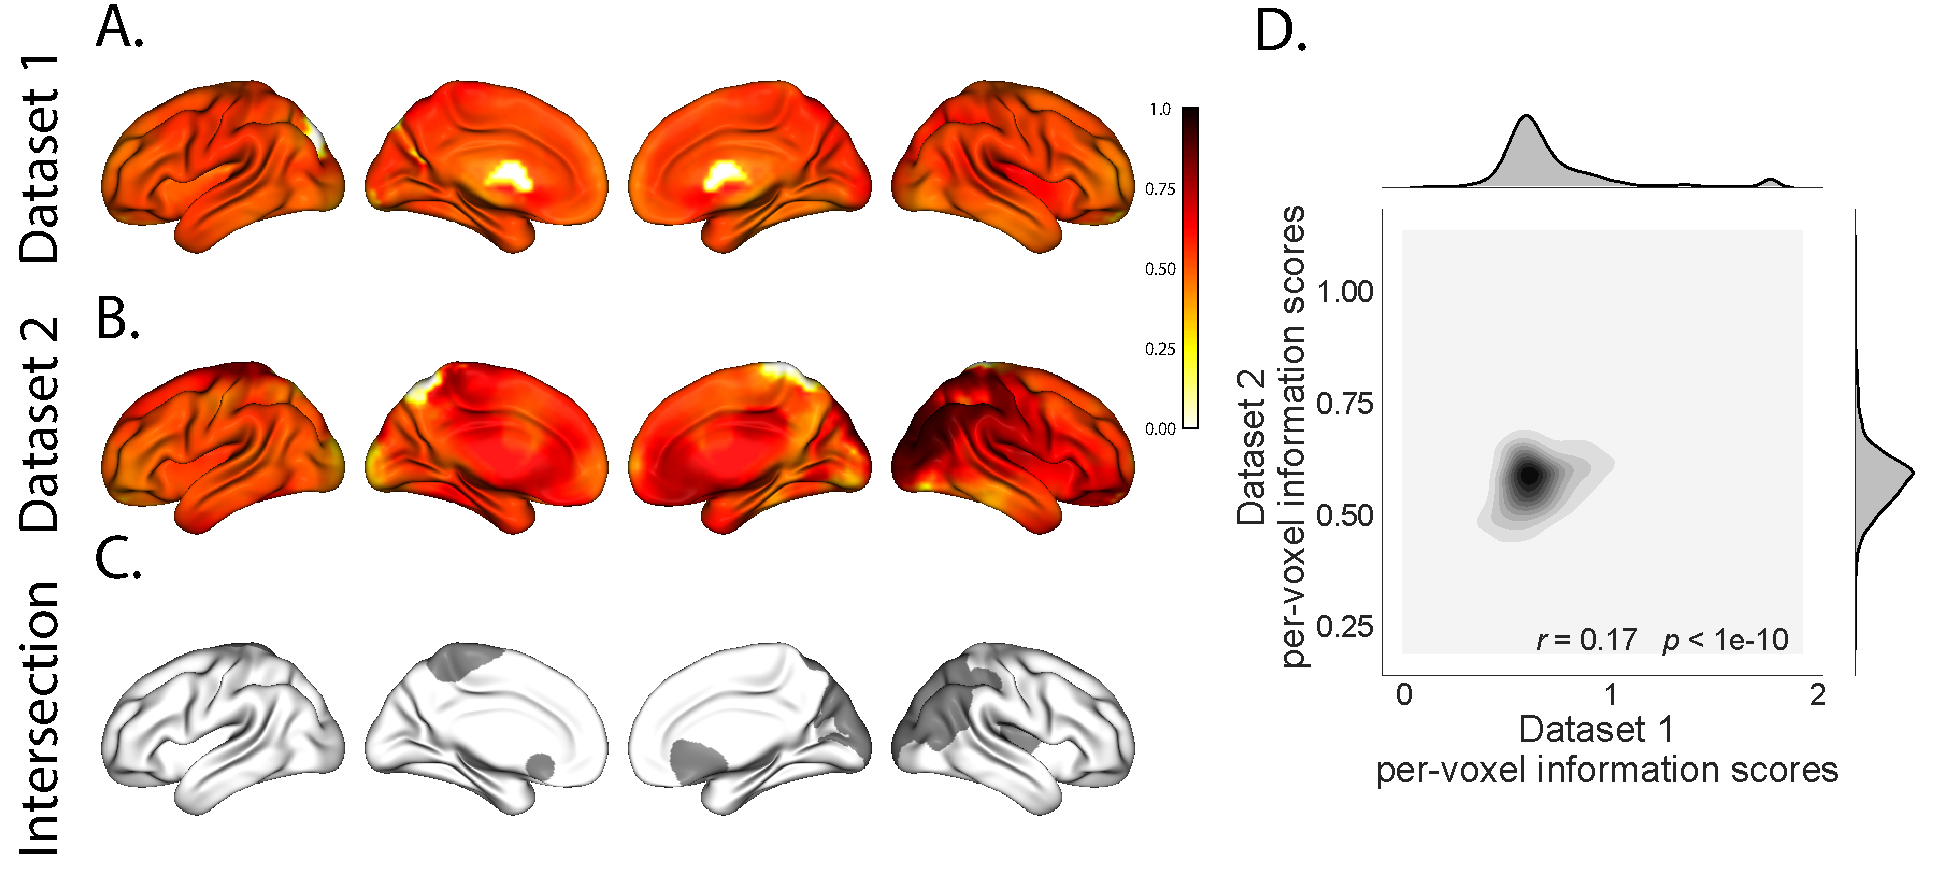
\includegraphics[width=\textwidth]{figs/informap}
  \caption{\textbf{Most informative electrode locations.}
    \textbf{A. Dataset 1 information score by voxel.} The voxel colors
    reflect the weighted average reconstruction accuracy across all
    electrodes from any patients with at least one electrode within 20
    MNI units of the given voxel.  \textbf{B. Dataset 2 information
      score by voxel.}  This panel is in the same format as Panel A.
    In both panels the contours indicate the intersections between the
    top 10\% most informative voxels in each map (also see
    Fig.~\networks Panels A.-C. All for networks within this region).  \textbf{C. Intersection.}  
    Gray areas indicate the intersections between the
    top 10\% most informative voxels in each map and projected onto the cortical surface~\citep{CombEtal19}. \textbf{D. Correspondence in information
      scores by voxel across Datasets 1 and 2.}  Same format as
    Figure~\ref{fig:density}C.}
  \label{fig:informap}
\end{figure}

We also wondered what frequency properties contributed to the
reconstruction accuracy. To recover frequency-band specific voltage activity
from each recording, a second-order Butterworth filter was applied
across bands $\delta$, $\theta$, $\alpha$, $\beta$, $\gamma_L$, and
$\gamma_H$ with respective frequency ranges 2-4 Hz, 4-8 Hz, 8-12 Hz,
12-30 Hz, 30-60 Hz, and 60-100 Hz. Bandpass signals contain
information about the phase and amplitude of the underlying frequency
band, providing the most detailed view of the activity at that
frequency. Additionally, we calculated the reconstruction accuracies
using power at each band by taking the absolute
value of the Hilbert tranform of the bandpassed signal (see Fig.~\freqpower). To compute the broadband power (BB), we
first computed instantaneous power at 50 log-spaced frequencies
between 2 and 100 Hz using Morlet wavelets (n=4). Then, for each time
point and electrode, we fitted a robust Huber regression to frequency
and power in log-space, and calculated the mean height of the
resulting line. We then followed the same procedure outlined above
(see Fig.~\ref{fig:methods}) to
obtain the reconstruction accuracy at each bandpassed frequency as well
as broadband power for both datasets (see Fig.~\ref{fig:frequency}).
We found
the best average reconstruction accuracy for each dataset was obtained using broadband
power, which is a correlate of neural firing
~\citep{MannEtal09}. We also found a similar trend in reconstruction
accuracy for frequency bands across the two datasets, performing better at lower
frequencies (peaking at $\alpha$) and worst at high frequencies (see Fig.~\ref{fig:frequency}).  

\begin{figure}
  \centering
  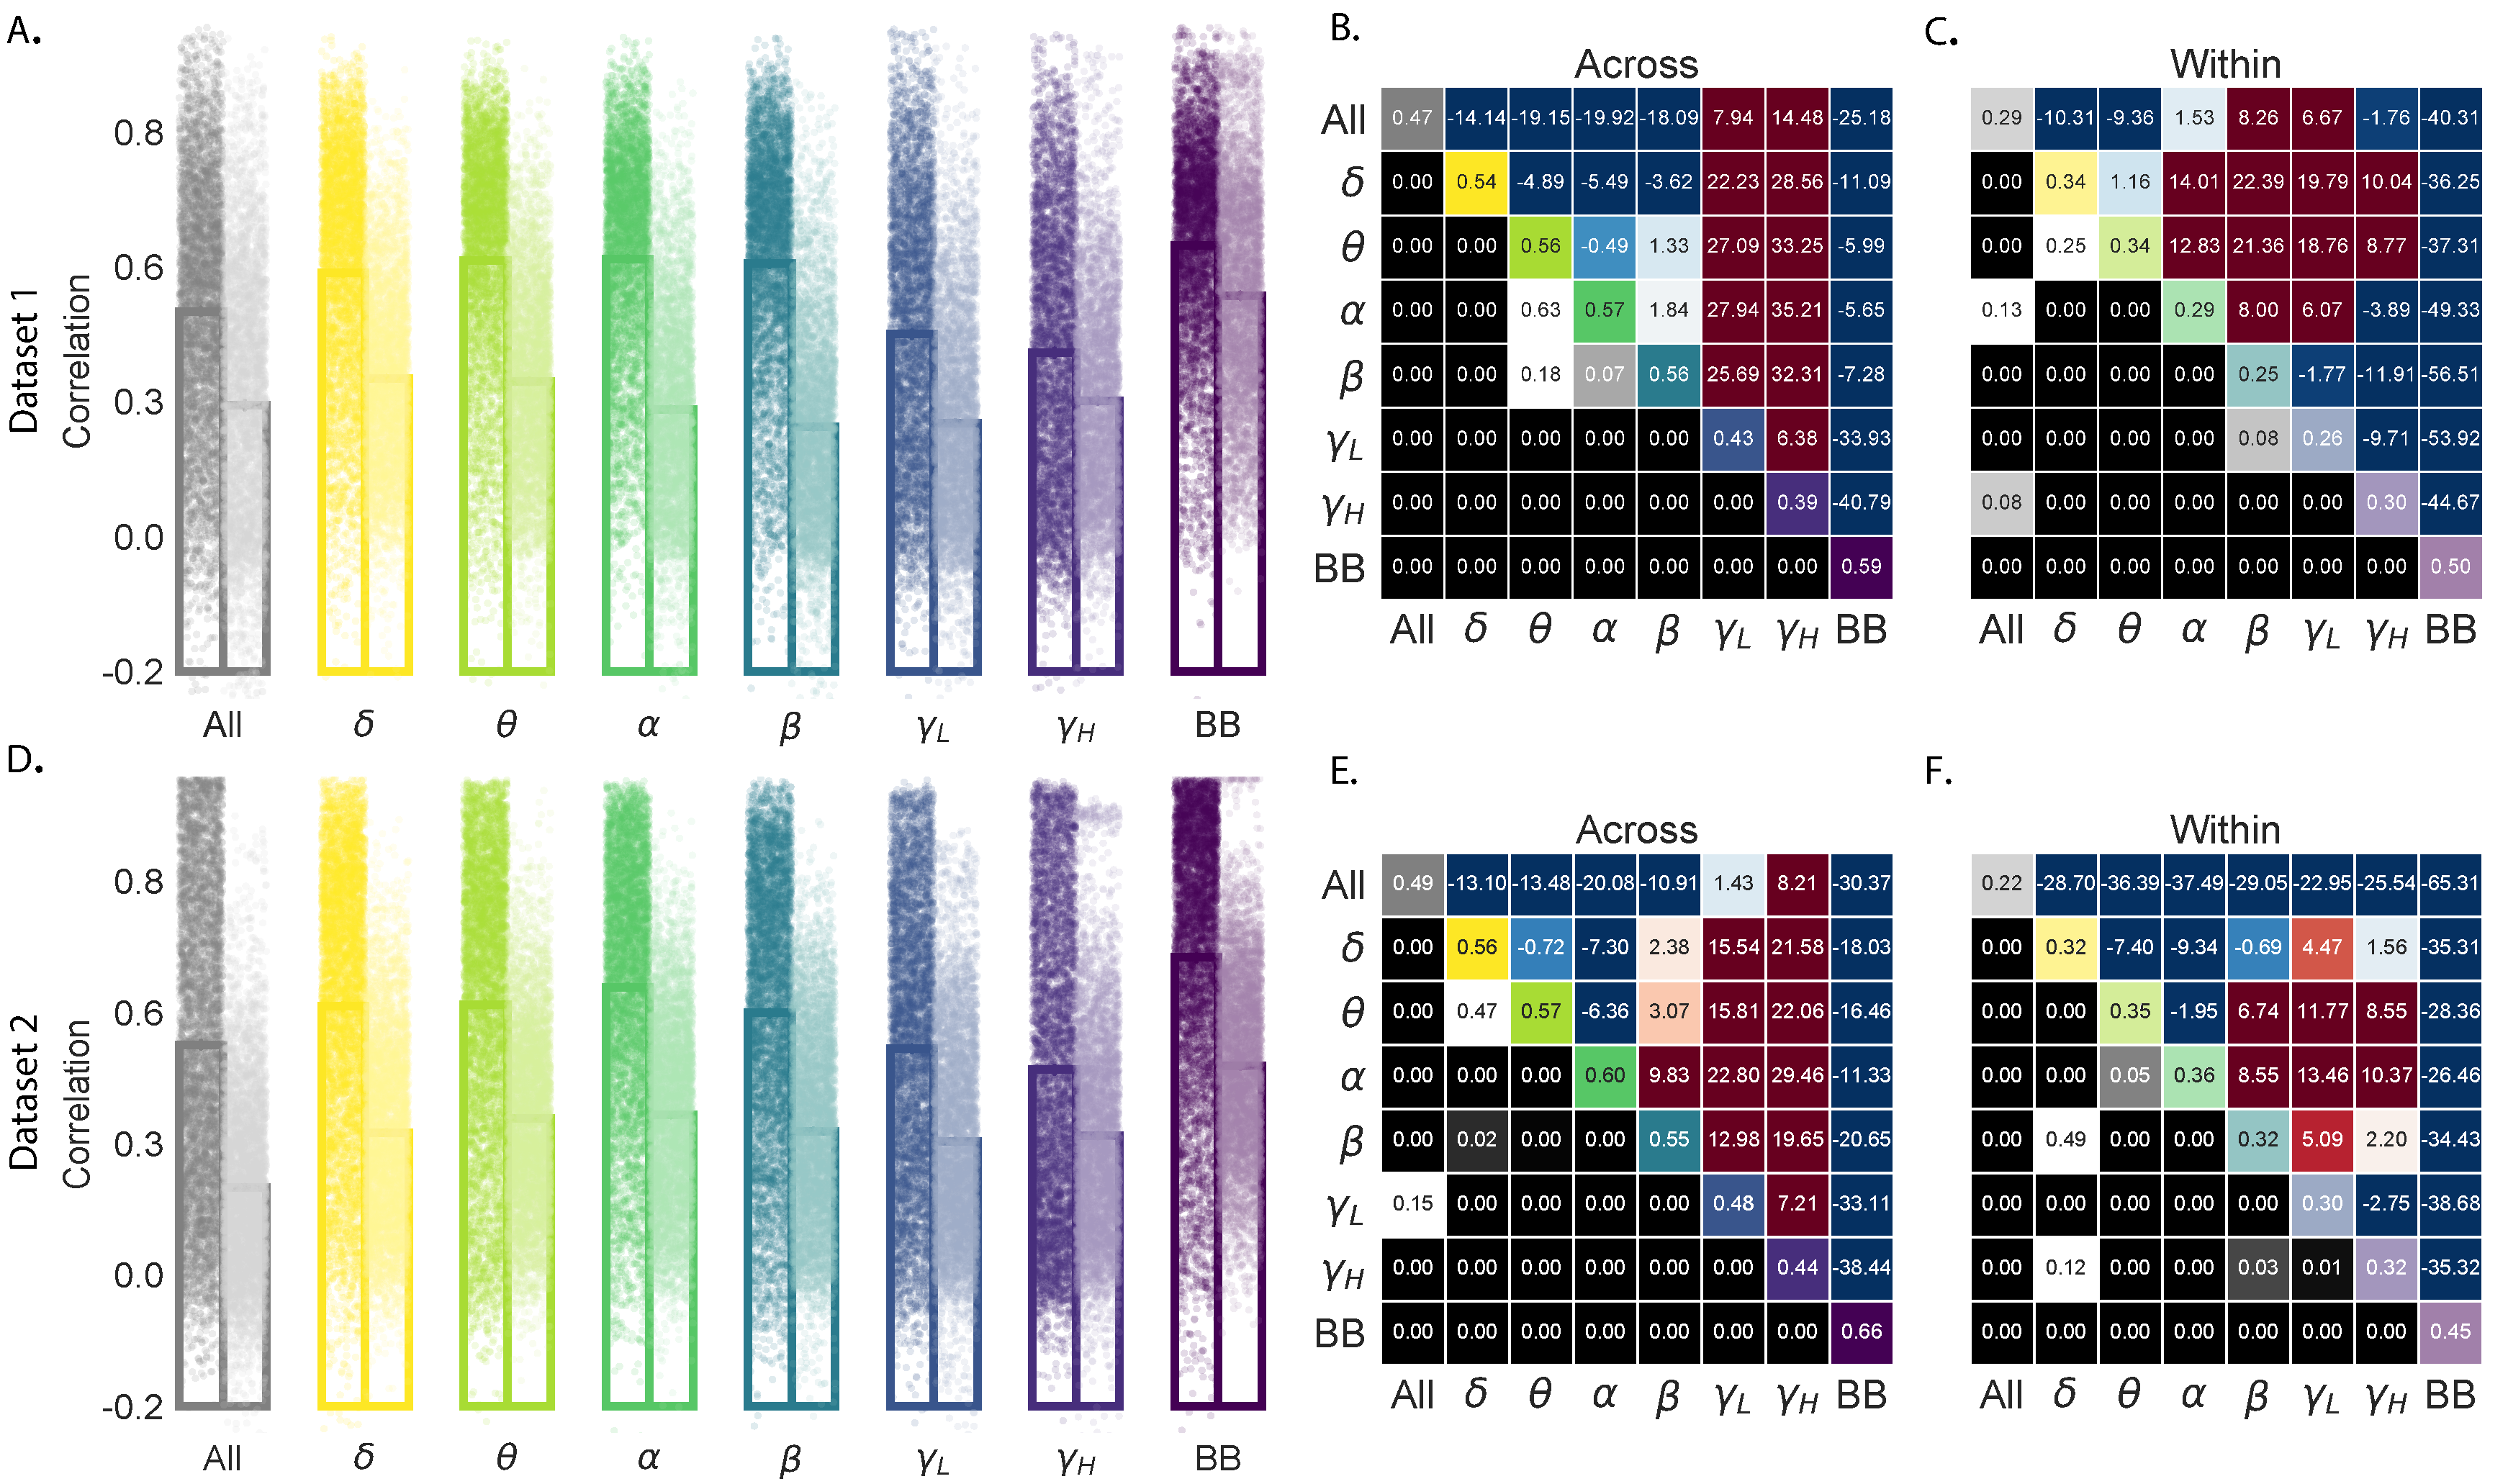
\includegraphics[width=\textwidth]{figs/frequency}
  \caption{\textbf{Reconstruction quality across all electrodes in two
      ECoG datasets for each frequency band.} \textbf{A. Distributions of correlations
      between observed versus reconstructed activity by electrode, for
      each frequency band in Dataset 1.}  The across-patient
    distribution (left jitter barplot) reflects
    reconstruction accuracy (correlation) using a correlation model
    learned from all but one patient's data, and then applied to that
    held-out patient's data.  The within-patient distribution (right
    jitter barplot in lighter color)
    reflects performance using a correlation model learned from the same
    patient who contributed the to-be-reconstructed electrode, colored
    by frequency and includes the raw voltages displayed in
    Fig.~\ref{fig:corrmap}A in gray.
    \textbf{B.~Statistical summary of across-patient reconstruction
      quality by electrode for each frequency band in Dataset 1.} In the upper triangles of each
    map, warmer colors (positive t-values) indicate that the
    distribution of
    reconstruction accuracy for the frequency band in a given row
    yielded was greater than the frequency band in the given
    column. Cooler colors (negative t-values) indicate that the
    frequency band in the given row yielded lower reconstruction
    accuracy than the frequency band in the given column. The lower
    triangles of each map denote the corresponding p-values for the
    t-tests. The diagonal entries display the average
    reconstruction accuracy given to each frequency
    band. \textbf{C.~Statistical summary of within-patient reconstruction
      quality by electrode for each frequency band in Dataset 1.}
    This panel displays the within-patient statistical summary,
    in the same format as Panel B.  \textbf{D.~Distributions of correlations
      between observed versus reconstructed activity by electrode, for
      each frequency band in Dataset 2.}  This panel displays
    reconstruction accuracy distributions for each frequency band for
    Dataset 2. \textbf{E.~Statistical summary of
      across-patient reconstruction quality by electrode for each
      frequency band in Dataset 2.} This is the same format as Panel
    B for Dataset 2. \textbf{F.~Statistical summary of
      within-patient reconstruction quality by electrode for each
      frequency band in Dataset 2.}This is the same format as Panel
    C for Dataset 2.}
  \label{fig:frequency}
\end{figure}

We also wanted to see how the most informative regions changed by
frequency. Lower frequency oscillations, such as $\delta$, $\theta$, and $\alpha$, have
been posited to be involved in processing modes which span large swaths of
cortical regions and are thought to serve the purpose of integration
across many cortical sites ~\citep{Knya12}. Higher frequency
oscillations such as $\beta$ and $\gamma$, are more limited to topographic
areas ~\citep{Nune95}, and are modulated by slow oscillations
hierarchically ~\citep{EngeEtal10}. Using the frequency-specific reconstruction accuracies, we
followed the process outlined in Fig.~\ref{fig:informap}C, to obtain
the most informative locations for each frequency.  When we examined the intersection
between the top 10\% most informative voxels across the two datasets
for each bandpassed frequency, we found a somewhat consistent hierarchical
structure (see Fig.~\ref{fig:networks}E).

We then wondered which
networks were involved in each of
these frequency-specific intersecting regions.  To better understand the networks involved
we colored the regions (Fig.~\ref{fig:networks}A) based on the
network parcellation ~\citep[using $k$=7;][]{YeoEtal11}} (Fig.~\ref{fig:networks}D) and calculated the proportion of each
of those networks (Fig.~\ref{fig:networks}B).  Consistent with the idea outlined
above, we found networks most involved in the lowest frequency band,
$\delta$, were networks involved integration and global processing
(specifically the dorsal attention ~\citep{MarzEtal13}, default mode,
and frontoparietal networks).  Although these networks are also seen
in the $\theta$ intersection, they are less proportionally to the
visual network.  Alpha power is consistently modulated in EEG studies
of attention and visuo-motor ~\citep{MantEtal07, MarzEtal13}, and we
similarly found a high proportion of visual, somatomotor, and dorsal attention networks
within this band.  We found $\beta$ intersections to predominantly
consist of somatomotor network, in line with~\citep{RittEtal09, VaneEtal11}.  Also accordant with heavily cited
literature~\citep{FrieEtal07}, the network most predominant in the
$\gamma$ intersection was the visual network.  Lastly, broadband power
was found predominantly in frontoparietal and default mode networks,
consistent with ~\citep{OssaEtal11}.

\begin{figure}
  \centering
  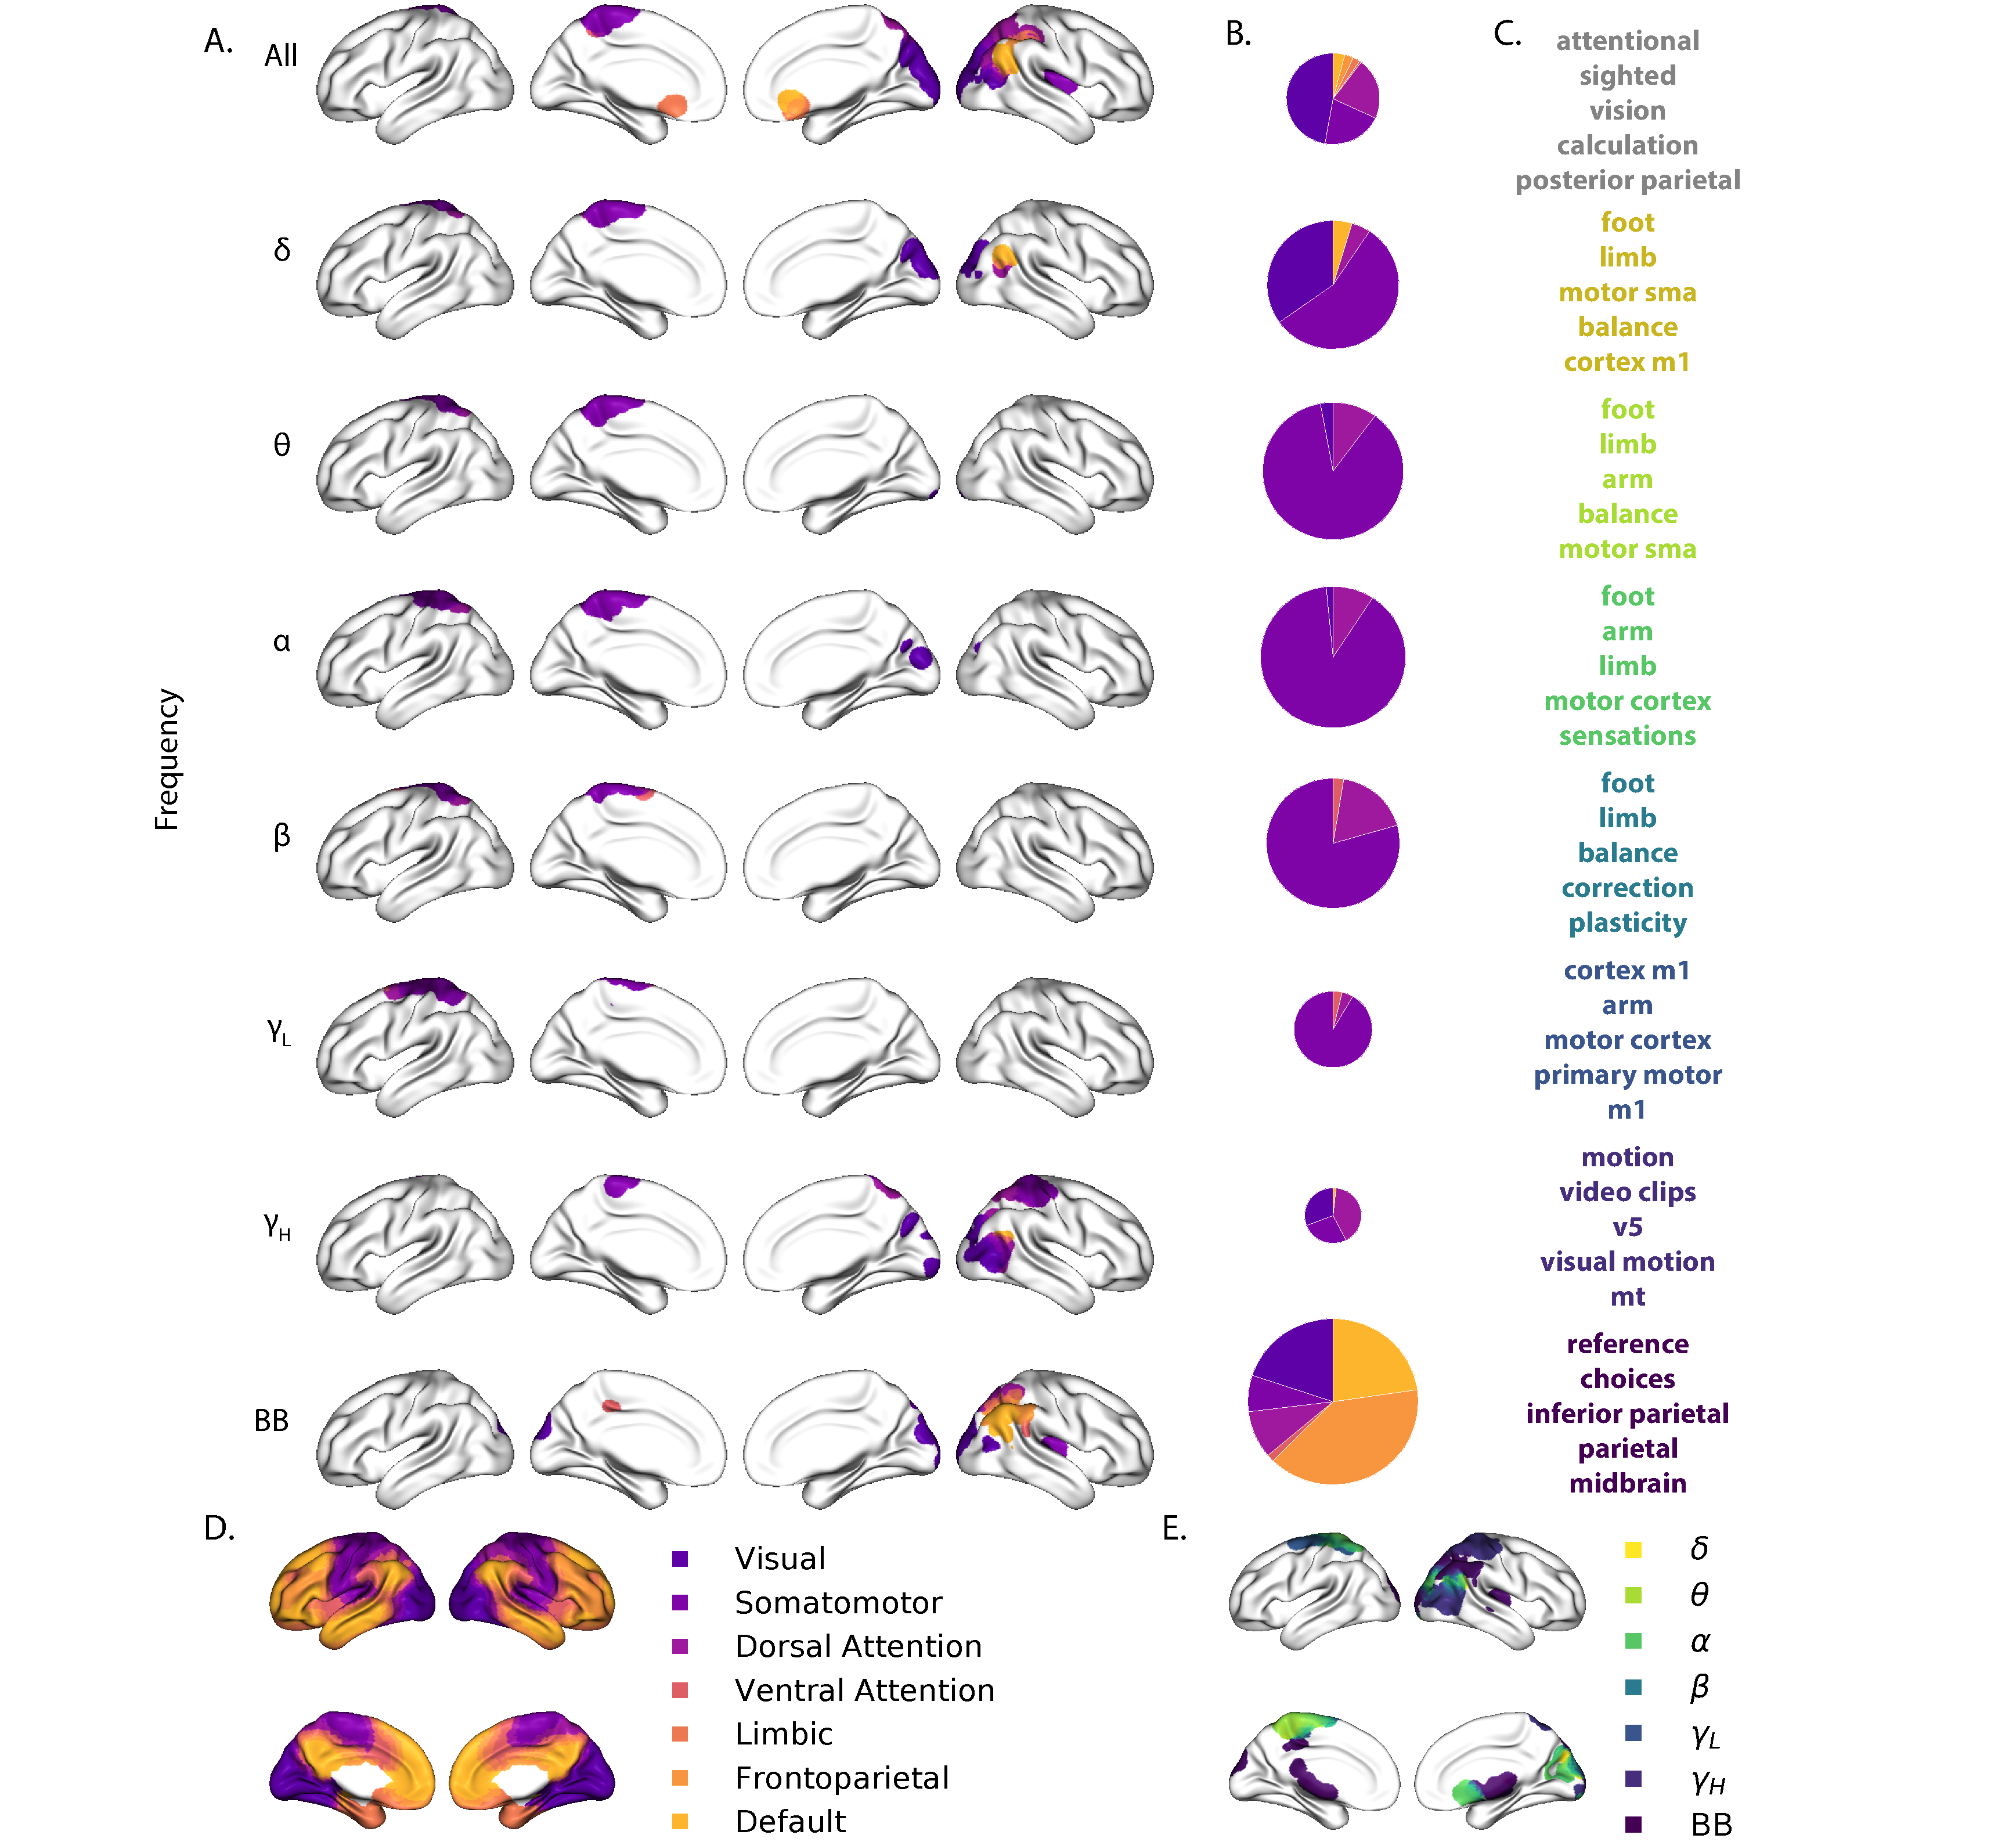
\includegraphics[width=\textwidth]{figs/networks}
  \caption{\textbf{Most informative electrode locations by frequency
      and the networks involved.}
    \textbf{A.~Intersections across datasets for each frequency.} The
    inflated brain plots display the intersections between the
    top 10\% most informative voxels were calculated as described in Fig.~\ref{fig:informap}
    for each frequency and projected onto the cortical surface~\citep{CombEtal19}. Intersecting voxels are colored according to the 7 networks
    from~\citep{YeoEtal11}.
    \textbf{B.~Proportion of networks in most informative electrode locations by
    frequency.}  Pie graphs display the proportion of the 7 networks
  ~\citep{YeoEtal11} in the most informative locations by
  frequency, and are sized relative to the average reconstruction
  accuracy for each frequency. \textbf{C.~Terms associated with most informative
    electrode locations.}  The
    lists of terms display the top five Neurosynth
    terms~\citep{RubiEtal17} decoded from the corresponding brain
    maps, and colored according the frequency (see Panel
    E legend). \textbf{D.~Network parcellation from~\citep{YeoEtal11}.}
    Seven network parcellation as described
    in~\citep{YeoEtal11}. \textbf{E.~Most informative locations by
      frequency.} The inflated brain plot displays the locations of
    the most informative locations (Panel A), colored by frequency,
    and projected onto the cortical surface~\citep{CombEtal19}.}
  \label{fig:networks}
\end{figure}



\section*{Discussion}
Are our brain's networks static or dynamic?  And to what extent are
the network properties of our brains stable across people and tasks?
One body of work suggests that our brain's \textit{functional}
networks are dynamic~\citep[e.g., ][]{MannEtal18},
person-specific~\citep[e.g., ][]{FinnEtal15}, and
task-specific~\citep[e.g., ][]{Turk13}.  In contrast, although the
gross anatomical structure of our brains changes meaningfully over the
course of years as our brains develop, on the timescales of typical
neuroimaging experiments (i.e., hours to days) our anatomical networks
are largely stable~\citep[e.g., ][]{CaseEtal00}.  Further, many
aspects of brain anatomy, including white matter structure, are largely
preserved across people~\citep[e.g., ][]{TalaTour88, JahaEtal13,
  MoriEtal08}. There are several possible means of reconciling this
apparent inconsistency between dynamic person- and task-specific
functional networks versus stable anatomical networks.  For example,
relatively small magnitude anatomical differences across people may be
reflected in reliable functional connectivity differences.  Along
these lines, one recent study found that diffusion tensor imaging
(DTI) structural data is similar across people, but may be used to
predict person-specific resting state functional connectivity
data~\citep{BeckEtal18}.  Similarly, other work indicates that
task-specific functional connectivity may be predicted by resting
state functional connectivity data~\citep{ColeEtal16, TavoEtal16}.  Another
(potentially complementary) possibility is that our functional
networks are constrained by anatomy, but nevertheless exhibit
(potentially rapid) task-dependent changes~\citep[e.g.,
][]{SporBetz16}.

Here we have taken a model-based approach to studying whether high
spatiotemporal resolution activity patterns throughout the human brain
may be explained by a static connectome model that is shared across
people and tasks.  Specifically, we trained a model to take in
recordings from a subset of brain locations, and then predicted
activity patterns during the same interval, but at \textit{other}
locations that were held out from the model.  Our model, based on
Gaussian process regression, was built on three general hypotheses
about the nature of the correlational structure of neural activity
(each of which we tested).  First, we hypothesized that functional
correlations are stable over time and across tasks.  We found that,
although aspects of the patients' functional correlations were
stable across tasks, we achieved better reconstruction accuracy when
we trained the model on within-task data~\citep[we acknowledge that
our general approach could potentially be extended to better model
across-task changes, following][and others]{ColeEtal16, TavoEtal16}.
Second, we hypothesized that some of the correlational structure of
people's brain activity is similar across individuals.  Consistent
with this hypothesis, our model explained the data best when we
trained the correlation model using data from \textit{other}
patients-- even when compared to a correlation model trained on the
same patient's data.  Third, we resolved ambiguities in the data by
hypothesizing that neural activity from nearby sources will tend to be
similar, all else being equal.  This hypothesis was supported through
our finding that all of the models we trained that incorporated this
spatial smoothness assumption predicted held-out data well above chance.

One potential limitation of our approach is that it does not provide a
natural means of estimating the precise timing of single-neuron action
potentials.  Prior work has shown that gamma band and broadband
activity in the LFP may be used to estimate the firing rates of
neurons that underly the population contributing to the
LFP~\citep{MillEtal08, MannEtal09, JacoEtal10b, CronEtal11}.  Because
SuperEEG reconstructs LFPs throughout the brain, one could in
principle use broadband power in the reconstructed signals to
estimate the corresponding firing rates (though not the timings of
individual action potentials). Interestingly, our frequency-specific
analysis yielded the best reconstruction accuracies using broadband
power.  

Beyond providing a means of estimating ongoing activity throughout the
brain using already implanted electrodes, our work also has
implications for where to place the electrodes in the first place.
Electrodes are typically implanted to maximize coverage of suspected
epileptogenic tissue.  However, our findings suggest that this
approach could be further optimized.  Specifically, one could leverage
not only the non-invasive recordings taken during an initial
monitoring period (as is currently done routinely), but also
recordings collected from other patients.  We could then ask: given
what we learn from other patients' data (and potentially from the
scalp EEG recordings of this new patient), where should we place a
fixed number of electrodes to maximize our ability to map seizure
foci?  As shown in Figures~\ref{fig:informap} and~\intersectmap, recordings from
different locations are differently informative in terms of
reconstructing the spatiotemporal activity patterns throughout the
brain.  This property might be leveraged in decisions about where to
surgically implant electrodes in future patients.

\section*{Concluding remarks}
Over the past several decades, neuroscientists have begun to leverage
the strikingly profound mathematical structure underlying the brain's
complexity to infer how our brains carry out computations to support
our thoughts, actions, and physiological processes.  Whereas
traditional beamforming techniques rely on geometric
source-localization of signals measured at the scalp, here we propose
an alternative approach that leverages the rich correlational
structure of two large datasets of human intracranial recordings.  In
doing so, we are one step closer to observing, and perhaps
someday understanding, the full spatiotemporal structure of human
neural activity.

\section*{Code availability}
We have published an open-source toolbox implementing the SuperEEG
algorithm.  It may be downloaded
\href{https://supereeg.readthedocs.io/en/latest/}{\underline{here}}. Additionally,
we have provided code for all analyses and figures reported in the
current manuscript, available
\href{https://github.com/ContextLab/supereeg_paper}{\underline{here}}.

\section*{Data availability}
The dataset analyzed in this study was generously shared by Michael
J. Kahana.  A portion of Dataset 1 may be downloaded
\href{http://memory.psych.upenn.edu/Request_EEG_access?paper=SedeEtal03}{\underline{here}}.
Dataset 2 may be downloaded
\href{http://memory.psych.upenn.edu/Request_EEG_access?paper=EzzyEtal17}{\underline{here}}.

\section*{Acknowledgements}
We are grateful for useful discussions with Luke J. Chang, Uri Hasson,
Josh Jacobs, Michael J. Kahana, and Matthijs van der Meer.  We are
also grateful to Michael J. Kahana for generously sharing the ECoG
data we analyzed in our paper, which was collected under NIMH grant
MH55687 and DARPA RAM Cooperative Agreement N66001-14-2-4-032, both to
M.J.K.  Our work was also supported in part by NSF EPSCoR Award Number
1632738 and by a sub-award of DARPA RAM Cooperative Agreement
N66001-14-2-4-032 to J.R.M.  The content is solely the responsibility
of the authors and does not necessarily represent the official views
of our supporting organizations.

\section*{Author Contributions}
J.R.M conceived and initiated the project. L.L.W.O., T.A.M, and
A.C.H. performed the analyses. J.R.M. and L.L.W.O. wrote the
manuscript.

\section*{Author Information}
Reprints and permissions information is available at www.nature.com/reprints.  The authors declare no competing financial interests.  Readers are welcome to comment on the online version of the paper.  Publisher's note: Springer Nature remains neutral with regard to jurisdictional claims in published maps and institutional affiliations.  Correspondence and requests for materials should be addressed to J.R.M. (jeremy.r.manning@dartmouth.edu).

\bibliography{CDL-bibliography/memlab}
\bibliographystyle{CSE}

\clearpage

\end{document}




















